\documentclass{article}

\PassOptionsToPackage{numbers, compress}{natbib}
\usepackage[preprint]{neurips_2025}

\usepackage[utf8]{inputenc}
\usepackage[T1]{fontenc}
\usepackage{hyperref}
\usepackage{url}
\usepackage{booktabs}
\usepackage{amsfonts}
\usepackage{amsmath}
\usepackage{amssymb}
\usepackage{nicefrac}
\usepackage{microtype}
\usepackage{xcolor}
\usepackage{graphicx}
\usepackage{multirow}

\title{DQN, PPO and MAPPO in Stag-Hunt 
\\ with Prosocial Reward Shaping}

\author{%
  Leonardo Benini\\
  Autonomous and Adaptive Systems, University of Bologna\\
  \texttt{leonardo.benini3@studio.unibo.it 1189330}
}

\begin{document}

\maketitle

\begin{abstract}
Stag Hunt is a simple game where the cooperative outcome pays best but is risky, and
there is a safe fallback that pays less. \citet{prosoc} showed that shaping each agent's
reward toward its partner makes cooperation easier to
learn, using two agents that learned with REINFORCE from pixels. We
redo this with three different deep RL algorithms: an independent value learner (DQN) and two
policy-gradient learners PPO and its CTDE variant MAPPO, on the three Gymnasium Stag-Hunt games,
sweeping how many of the two agents are prosocial, over three seeds. Shaping helps
different learners in different games. DQN on stag hunt reaches the cooperative equilibrium
with two prosocial learners, while PPO and MAPPO require at least one for escalation.
No model reaches the optimal strategy in stag hunt, which is to walk towards the stag together
while foraging for plants.
\end{abstract}

\section{Introduction}

Getting self-interested learners to cooperate is a recurring problem in multi-agent
reinforcement learning (MARL). A simple environment to study it is the Stag Hunt: two hunters each
decide whether to go after a stag, which needs both of them, or to forage for plants alone.
Hunting the stag together is best for both, but risky, because a hunter who commits to the
stag while the other does not gets nothing, or is punished. Foraging for plants is safe.
Independent learners, each treating the other as part of the environment, tend to end up at
the safe outcome \citep{prosoc}.

\citet{prosoc} suggest to induce cooperation with prosocial reward shaping, 
giving each agent a reward that is partly its partner's.
\begin{equation}
  U_i \;=\; (1-\alpha_i)\, r_i \;+\; \alpha_i\, r_j ,
  \label{eq:prosocial}
\end{equation}
so that for $\alpha>0$ an agent partly cares about the other's payoff, which makes the
cooperative equilibrium easier to reach. Their agents share one convolutional network and
learn with REINFORCE from pixels. We check whether this still works with three different algorithms:
a modern implementation of DQN with target networks, PPO and its CTDE variant MAPPO, comparing them to determine
whether it is the type of learner(value vs policy), the centralised critic or the reward shaping that matters more for coordination.

We also ignore parameter sharing, so each agent has its own networks and coordination has to be
learned rather than coming for free from identical policies, except for the critic in MAPPO naturally, and we keep the true rewards so
the risk that defines the stag hunt is not removed by clipping.

\section{Environments}
\label{sec:envs}

We use the three \texttt{gymnasium-stag-hunt} Markov games. Each is a two-agent $5\times5$
gridworld with five actions (four moves and stand) and a 250-step (Hunt, Harvest) or 50-step
(Escalation) horizon. They only end by running out of time, and returns below are the
sum of both agents' unshaped returns.
From the beginning, set penalty values were chosen from the sweeps in \citet{prosoc} to be on the harder side.

\paragraph{Hunt.} One stag, two plants. Catching the stag together pays $+5$ to both.
Stepping onto the stag alone is a mauling and pays a penalty $g$ (we use $g=1$). Foraging a
plant pays $+1$ to the forager. The stag walks toward the nearest agent and stays put after
mauling, so an agent that approaches it alone gets punished repeatedly. Both hunting is the
good but risky equilibrium; both foraging is the safe one.

\paragraph{Escalation.} A single marker tile appears. On each step where both agents stand on
it, both get $+1$ and a shared streak counter goes up. If one agent leaves while the other
stays, the one that leaves breaks the streak and is punished by $-0.5$ times the streak
length. Cooperation is easy to start but gets more expensive to abandon, so it tests
coordination that has to be kept up over time.

\paragraph{Harvest.} Plants are young or mature. Harvesting a young plant pays $+1$ to the
harvester only; waiting for it to mature pays $+2$ to both. Plants mature and die at random,
tuned so a plant lives about 20 steps on average. An average chance to mature of 30\% is used, on the harder side of the default 50\%.


\section{Method}
\label{sec:method}

\paragraph{Observations.} The environments can return an RGB image
or a short coordinate vector (positions of the agents, the stag or mark, and the plants). We
train on the coordinate vector, scaled to $[0,1]$. In a fully
observable $5\times5$ grid the image and the coordinate vector hold the same information, and
recovering one from the other is easy by template matching against the few sprites. A trivial 
single kernel CNN(with specific size and side) could also be used, either trained separately or end-to-end. To evaluate many different learners and enviroments we train
directly from the coordinates with a small MLP, which is significantly faster.

\paragraph{Algorithms.} \textbf{DQN} is independent Double
DQN \citep{ddqn2016}: one online and one target Q-network $Q_i(o_i;\theta_i)$ per agent
(two-layer ReLU MLP, width 64), $\varepsilon$-greedy with a linear anneal, a smooth-$L_1$ loss, and a
shared replay buffer where each agent trains only on its own column. \textbf{PPO}
is \citep{ppo2017} implemented by following the 37 details \citep{ppo37}, most notably: separate
tanh-MLP actor and critic with orthogonal init, GAE($\lambda$) \citep{gae2016} with correct
bootstrapping at the time limit, clipped policy and value losses, per-mini-batch advantage
normalisation, an entropy bonus, KL early stopping, and rollouts from $N$ parallel
environments. Following \citet{mappo2021} we normalise the value targets, which keeps the
value loss at a stable scale and lets us train on the true reward without clipping. \textbf{MAPPO}
changes only the critic: its single centralised critic sees the concatenated observation
$[o_0,o_1]$ and is trained on both agents' returns, while PPO keeps a separate critic
$V_i(o_i)$ per agent. The actors are independent in both, so PPO versus MAPPO isolates the
centralised critic. Some of the suggested improvement in \citet{mappo2021} like value normalization are also applied to PPO.

\paragraph{Reproducibility.} We seed Python, NumPy, TensorFlow and
Keras' initialiser together, disable oneDNN reduction reordering, and enable deterministic ops
to make sure runs are fully reproducible.

\section{Experimental setup}
\label{sec:setup}

The full run is 3 games $\times$ 3 algorithms $\times$ 3 prosociality settings $\times$ 3
seeds $=$ 81 runs. Step budgets are 400k (Hunt), 500k (Escalation) and 1M (Harvest), enough
for every curve to stabilize. The PPO learners use $N=8$ parallel environments on Hunt and
$N=16$ on Harvest; DQN runs single-stream, since parallel environments do not help given the 
usage of a replay buffer. Exploration values and annealment schedules were selected via grid
search based on seed convergence and better returns. Everything runs on CPU (tiny MLPs) and single-threaded runs
are dispatched concurrently across all cores to maximize CPU utilization.
We report the joint return averaged over the last 20\% of each run's episodes, then over the
three seeds.

\newpage

\section{Results}
\label{sec:results}

\begin{table}[t]
  \centering
  \small
  \caption{Converged joint return (mean $\pm$ std over 3 seeds). Columns: both
  selfish, one prosocial, both prosocial.}
  \label{tab:results}
  \begin{tabular}{@{}ll ccc@{}}
    \toprule
    & & \multicolumn{3}{c}{Joint return (mean $\pm$ std)} \\
    \cmidrule(lr){3-5}
    Game & Algo & selfish & one pro. & both pro. \\
    \midrule
    \multirow{3}{*}{Hunt}
      & DQN  & $160.9\pm0.9$ & $154.3\pm1.2$ & $\mathbf{585.7\pm1.5}$ \\
      & PPO  & $588.1\pm12.8$ & $594.5\pm5.5$ & $597.8\pm2.9$ \\
      & MAPPO & $570.6\pm27.9$ & $587.8\pm7.3$ & $596.7\pm1.2$ \\
    \midrule
    \multirow{3}{*}{Escalation}
      & DQN  & $83.9\pm0.1$ & $83.9\pm0.0$ & $83.7\pm0.1$ \\
      & PPO  & $53.4\pm1.1$ & $\mathbf{90.2\pm0.3}$ & $89.5\pm0.8$ \\
      & MAPPO & $55.5\pm1.3$ & $90.0\pm0.3$ & $\mathbf{90.2\pm0.3}$ \\
    \midrule
    \multirow{3}{*}{Harvest}
      & DQN  & $594.9\pm8.7$ & $599.4\pm4.9$ & $594.9\pm7.5$ \\
      & PPO  & $629.3\pm1.1$ & $630.1\pm2.4$ & $629.3\pm1.2$ \\
      & MAPPO & $631.3\pm4.7$ & $626.9\pm1.4$ & $626.3\pm2.4$ \\
    \bottomrule
  \end{tabular}
\end{table}

\paragraph{Hunt.} DQN stays in the safe forage equilibrium when at least one agent is selfish
(160.9 and 154.3) and only reaches the stag when both agents are prosocial (585.7, all three
seeds). The PPO learners reach the stag at every setting. A fine grid search fo exploration schedules was tested and
none was found that enabled DQN to reach the stag with zero or one prosocial agent. The fully shared reward
in the case of both agents is enough to make them try to hunt for the stag, eventually learning to cooperate correctly.
PPO learners are much quicker to reach cooperation, regardless of shaping.

\paragraph{Escalation.} DQN achieves around the maximum joint reward of 100, scoring about 84 
in every run. The PPO learners are instead only able to apporach the maximum when at least one agent is prosocial. 
The slightly higher return of PPO learners is from the fact that they are quicker to start following the stag after an episode reset.

\paragraph{Harvest.} Because the mature harvest already pays both agents, their interests line
up without shaping, and all three learners reach the mutual-patience outcome (about 595 for
DQN, about 628 for PPO) with no real dependence on prosociality.

\begin{figure}[t]
  \centering
  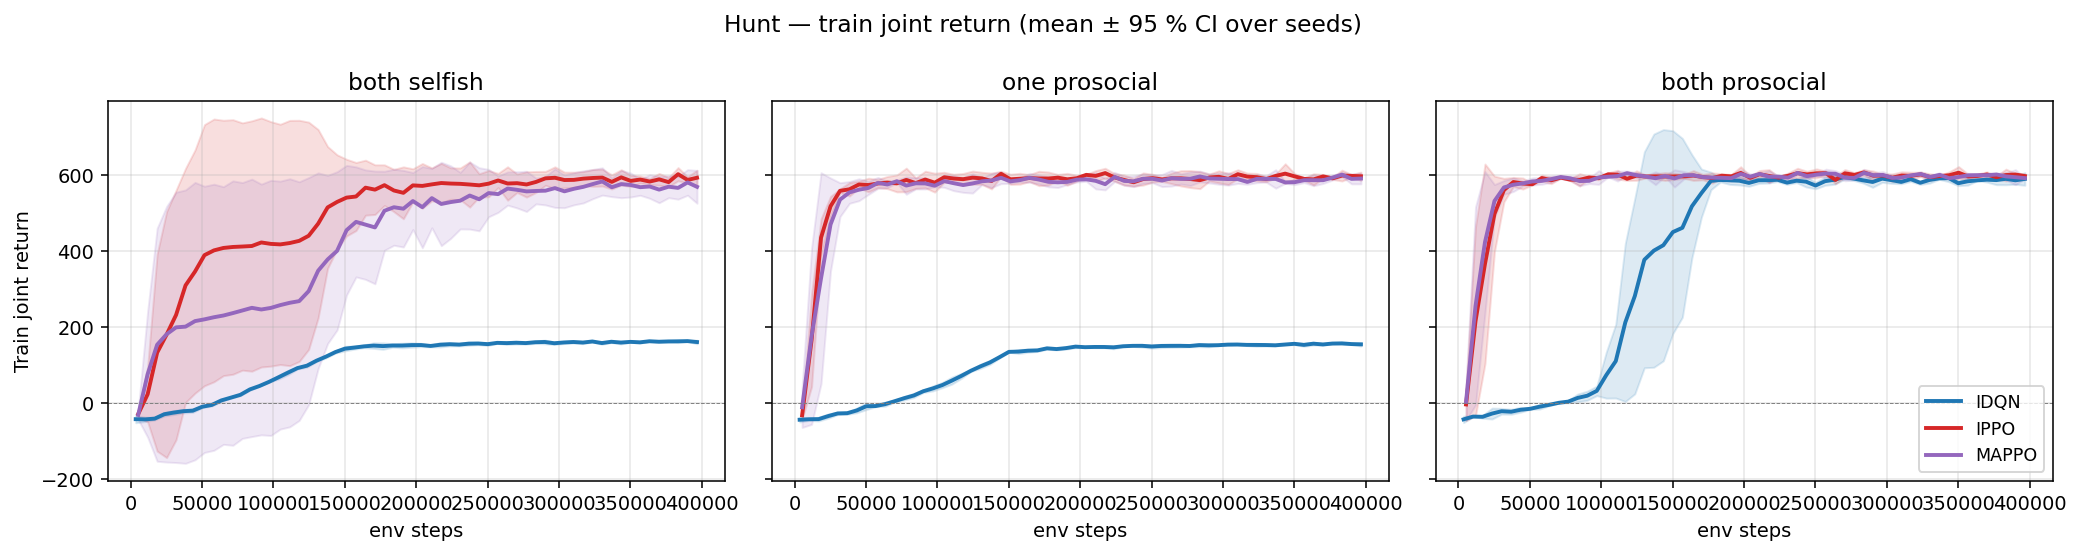
\includegraphics[width=0.78\linewidth]{figures/learning_curves_Hunt.png}\\[2pt]
  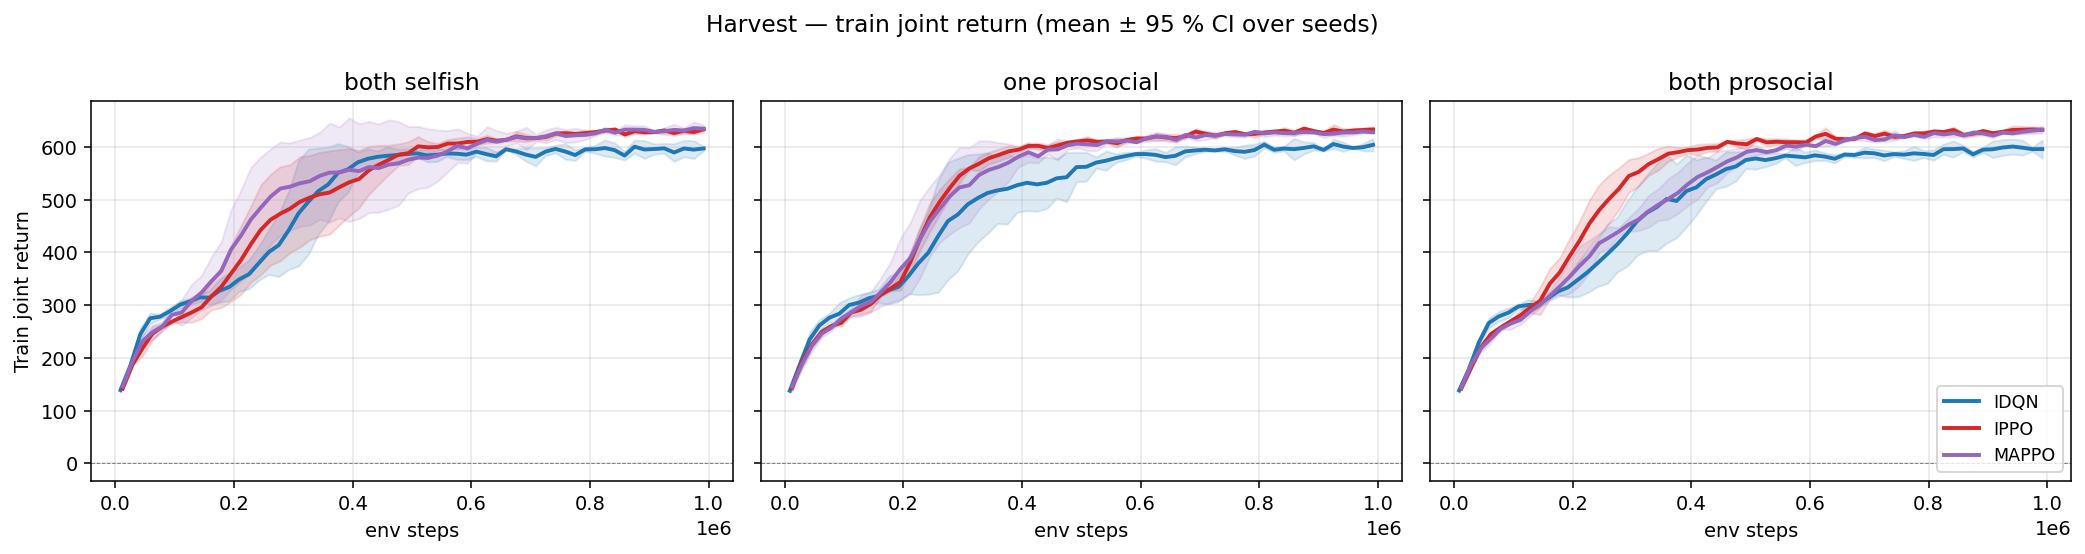
\includegraphics[width=0.78\linewidth]{figures/learning_curves_Harvest.png}
  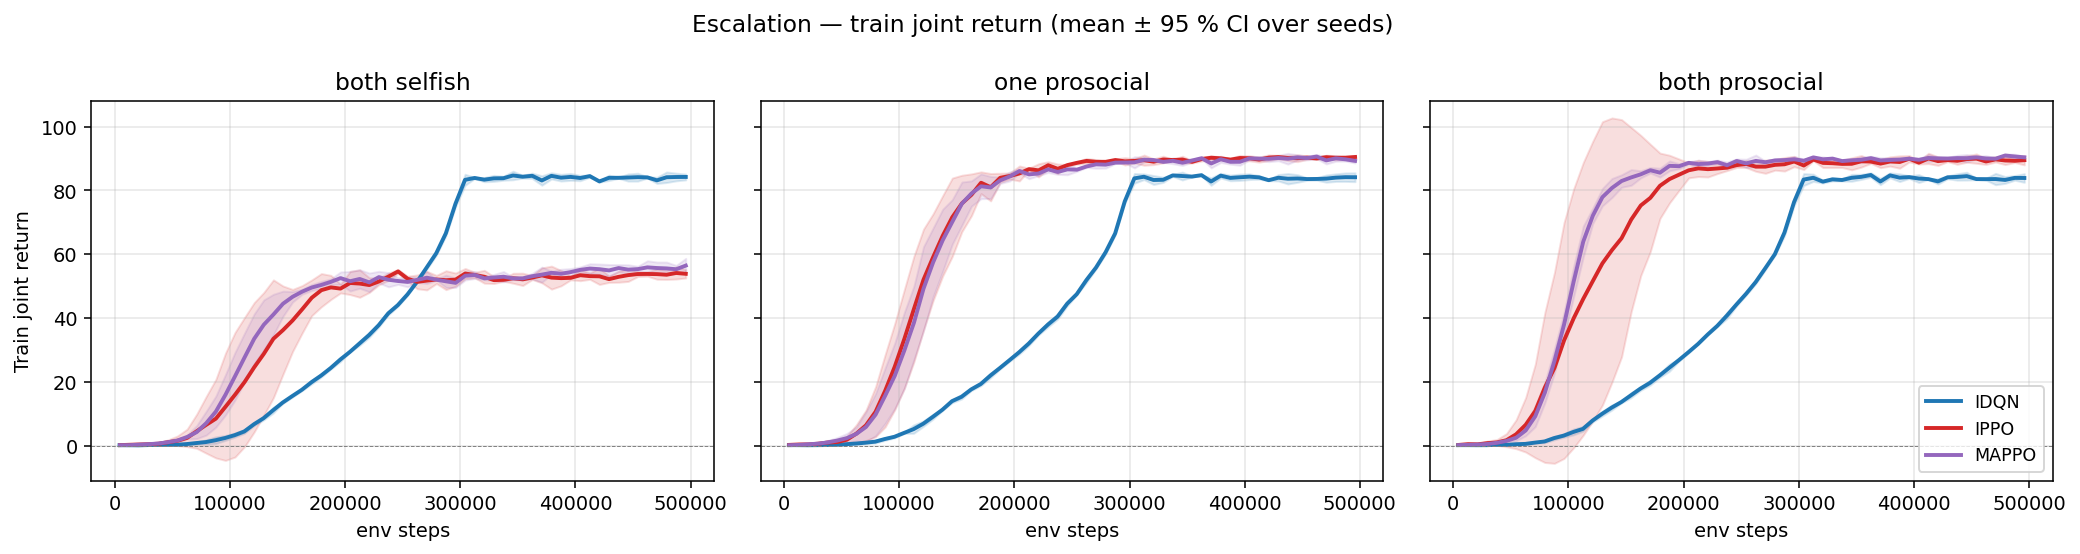
\includegraphics[width=0.78\linewidth]{figures/learning_curves_Escalation.png}
  \caption{Joint return (mean and 95\% CI over seeds) against steps, one panel per prosociality
  setting. Top (Hunt): DQN (blue) stays at about 160 unless both agents are prosocial, then
  jumps to the stag at about 586; PPO (red) and MAPPO (purple) reach the stag everywhere.
  Bottom (Escalation): selfish PPO stalls at about 54 and shaping lifts it to about 90, while
  DQN reaches about 84 in every panel.}
  \label{fig:curves}
\end{figure}

\paragraph{PPO vs MAPPO.} There is no significant difference between the two learners.
Although PPO already maximizes the return for most configurations, we would expect MAPPO to perform better
in Escalation with both selfish agents, because the centralised critic sees both observations and can learn that the
  best action is to stay on the marker tile. However, the results show that both PPO and MAPPO achieve similar returns in this configuration, suggesting that the centralised critic does not provide a significant advantage in this case.

\paragraph{Suboptimal Hunt strategy.} Watching the trained Hunt agents in a rendered 
demo environment shows a limit for all learners. Every run that reaches the stag, both the DQN
both-prosocial runs and all the PPO runs, does it the same lazy way: the two agents move to the
same spot, usually a corner, and wait for the stag, which always steps toward the nearest agent
and so walks into them and is caught over and over. This gives a high return but is not the best
policy. None of the runs found the strategy a person would probably think of, chasing the stag together and
picking up the $+1$ plants on the way. Once corner-camping reliably brings in the $+5$s there is
no pressure to learn the harder forage-while-hunting policy, and the plant rewards are small next
to the stag rewards. So the agents find the good equilibrium but not the best policy overall.

\newpage 
\section{Conclusion}

Redoing the prosocial Stag-Hunt experiment with different, more sophisticated methods shows how
prosociality is never hurtful, but its impact is limited to only a handful of scenarios, with modern PPO 
methods performing generally well on all configurations. Prosociality is seen to help learners that are stuck
in a suboptimal equilibrion to reach the better one. DQN needs it to take the risky joint action on Hunt, 
PPO needs it
to commit on Escalation, and where the agents' interests already agree (Harvest) it does almost
nothing.  

Overall, the type of learner (value or policy) matters more than prosociality and whether the critic is
centralised, which barely mattered with two similar agents and small observations and would
likely matter more with more agents or partial observability. Finally, even when the agents reach the
cooperative equilibrium they often settle for a lazy corner-camping policy, so finding the right
equilibrium is not the same as playing optimally. 



\small
\setlength{\bibsep}{1pt plus 0.3ex}
\bibliographystyle{plainnat}
\begin{thebibliography}{9}
\setlength{\itemsep}{0pt}
\setlength{\parskip}{0pt}

\bibitem[Peysakhovich and Lerer(2017)]{prosoc}
A.~Peysakhovich and A.~Lerer.
\newblock Prosocial learning agents solve generalized stag hunts better than selfish ones.
\newblock \emph{arXiv:1709.02865}, 2017.

\bibitem[van Hasselt et al.(2016)]{ddqn2016}
H.~van Hasselt, A.~Guez, and D.~Silver.
\newblock Deep reinforcement learning with double Q-learning.
\newblock In \emph{AAAI}, 2016. arXiv:1509.06461.

\bibitem[Schulman et al.(2017)]{ppo2017}
J.~Schulman, F.~Wolski, P.~Dhariwal, A.~Radford, and O.~Klimov.
\newblock Proximal policy optimization algorithms.
\newblock \emph{arXiv:1707.06347}, 2017.

\bibitem[Schulman et al.(2016)]{gae2016}
J.~Schulman, P.~Moritz, S.~Levine, M.~Jordan, and P.~Abbeel.
\newblock High-dimensional continuous control using generalized advantage estimation.
\newblock \emph{arXiv:1506.02438}, 2016.

\bibitem[Yu et al.(2021)]{mappo2021}
C.~Yu, A.~Velu, E.~Vinitsky, J.~Gao, Y.~Wang, A.~Bayen, and Y.~Wu.
\newblock The surprising effectiveness of PPO in cooperative multi-agent games.
\newblock \emph{arXiv:2103.01955}, 2021.

\bibitem[Huang et al.(2022)]{ppo37}
S.~Huang et al.
\newblock The 37 implementation details of proximal policy optimization.
\newblock \emph{ICLR Blog Track}, 2022.

\end{thebibliography}

\end{document}
